\documentclass[review]{elsarticle}

\usepackage{lineno,hyperref}
\modulolinenumbers[5]

\journal{To Discuss With FIT Collaboration}

%%%%%%%%%%%%%%%%%%%%%%%
%% Elsevier bibliography styles
%%%%%%%%%%%%%%%%%%%%%%%
%% To change the style, put a % in front of the second line of the current style and
%% remove the % from the second line of the style you would like to use.
%%%%%%%%%%%%%%%%%%%%%%%

%% Numbered
%\bibliographystyle{model1-num-names}

%% Numbered without titles
%\bibliographystyle{model1a-num-names}

%% Harvard
%\bibliographystyle{model2-names.bst}\biboptions{authoryear}

%% Vancouver numbered
%\usepackage{numcompress}\bibliographystyle{model3-num-names}

%% Vancouver name/year
%\usepackage{numcompress}\bibliographystyle{model4-names}\biboptions{authoryear}

%% APA style
%\bibliographystyle{model5-names}\biboptions{authoryear}

%% AMA style
%\usepackage{numcompress}\bibliographystyle{model6-num-names}

%% `Elsevier LaTeX' style
\bibliographystyle{elsarticle-num}

\usepackage[acronym]{glossaries}
\newacronym{BU}{BU}{Burn up}
\newacronym{FLM}{FLM}{Fuel Loading Model}
\newacronym{FF}{FF}{Fixed Fraction}
\newacronym{BOC}{BOC}{Beginning of Cycle}
\newacronym{EOC}{EOC}{End of Cycle}
\newacronym{PWR}{PWR}{Pressurized Water Reactor}
\newacronym{SFR}{SFR}{Sodium Fast Reactor}
\newacronym{MOX}{MOX}{Mixed OXide}
\newacronym{UOX}{UOX}{Uranium OXide}
\newacronym{FIT}{FIT}{Functionality Isolation Test}


%%%%%%%%%%%%%%%%%%%%%%%

\begin{document}

\begin{frontmatter}

\title{Analysis Of Fuel Loading Management in Fuel Cycle Simulation Tools In The Framework Of The FIT Project}
%\tnotetext[mytitlenote]{Fully documented templates are available in the elsarticle package on \href{http://www.ctan.org/tex-archive/macros/latex/contrib/elsarticle}{CTAN}.}

%% Group authors per affiliation. 
% Rules for Author List : Two groups 
% Group 1 = Main contributors (calculations and/or significative helping writing)
% Group 2 = Other membre of the FIT Project
% Main writer is Corresponding Autor

% Group 1

\author[IPNO]{X.~Doligez}
\author[ANL]{B.~Feng}
\author[BUD]{M.~Halasz}
\author[SCK]{A.~Hernandez}
\author[MAULE]{I.~Merino}
\author[MAD]{B.~Mouginot}
\author[CIEMAT]{A.V.~Skarbeli}

\author[SUB]{N. Thiolli\`ere \corref{cor1}}
\ead{nicolas.thiolliere@subatech.in2p3.fr}

% Group 2
\author[CIEMAT]{F.~Alvarez-Velarde}
\author[ORNL]{E.~E.~Davidson}
\author[TRACT]{H.~Druenne}
\author[IPNO]{M.~Ernoult}
\author[INL]{R.~Hays}
\author[UI]{K.~Huff}
\author[BUD]{M.~Szieberth}
\author[TRACT]{B.~Vermeeren}
\author[CIEMAT]{A.~Villacorta}
\author[MAD]{P.~Wilson}

\cortext[cor1]{Corresponding author}

\address[IPNO]{Institut de Physique Nucléaire d’Orsay, CNRS-IN2P3/Univ, Paris-Sud, France}
\address[ANL]{Argonne National Laboratory, 9700 Cass Ave., Lemont, IL 60439, USA}
\address[BUD]{Budapest University of Technology and Economics (BME), Institute of Nuclear Techniques, 1111 Budapest, Müegyetem rkp. 3-9, Hungary}
\address[SCK]{Studiecentrum voor kernenergie - Centre d'étude de l'énergie nucléaire (SCK-CEN), Boeretang 200, Mol, Belgium}
\address[MAULE]{Catholic University of the Maule, Av. San Miguel 3605, Talca, Chile}
\address[MAD]{Univ. of Wisconsin Madison, Department of Nuclear Engineering and Engineering Physics, Madison, WI, United States}
\address[SUB]{Subatech, IMTA-IN2P3/CNRS-Universit\'e, Nantes, F-44307, France}
\address[ORNL]{Oak Ridge National Laboratory, Building 5700, Mail Stop 6172, Oak Ridge, TN 37831, United States}
\address[TRACT]{Tractebel Engie, Boulevard Simón Bolívar 34-36, 1000 Brussels, Belgium}
\address[INL]{Idaho National Laboratory, 2525 Fremont Ave., Idaho Falls, ID 83402, USA}
\address[UI]{University of Illinois, Department of Nuclear, Plasma, and Radiological Engineering, United States}
\address[CIEMAT]{CIEMAT, Avda. Complutense, 40, 28040 Madrid, Spain}

\begin{abstract}
Abstract beginning...


In this paper, the first tested functionality is presented. The impact of the fuel composition dependency with stock versus a fixed fraction approach is tested. Results from different methodologies are compared.
\end{abstract}

\begin{keyword}
Nuclear Fuel Cycle \sep Simulation \sep Functionality \sep Benchmark
\end{keyword}

\end{frontmatter}

\linenumbers

% #########################################################################################
% #########################################################################################
% #########################################################################################

Since the 1990's, many different nuclear fuel cycle simulators have been
developed by several institutions.

A fuel cycle simulator aims to models an entire nuclear fleet including main
facilities, such as nuclear reactors, fuel fabrication plants, reprocessing
plants, cooling pool and/or waste disposal. Those tools help to identify drivers
and interactions between parameters in fuel cycle. They implement physic models
for different key points of the cycle such as fuel fabrication or burn up
depletions, with various level of complexicity. 

Fuel cycle simulator are used worldwide for wide range of applications:
optimisation of the industrial operation of a existing nuclear fleet, assessing
the future of nuclear energy and providing valuable informations required for
the political decision, evaluation/verification of the operation of an exisiting
nuclear fleet by national or international safety authorities. Moreover, those
tools are used for Research and Development training as access point to key
datas related to the fuel cycle. 

The different institutions that use (and develop) fuel cycle simulators pursue
different goals. Consequently, the level of rafinment of each software pieces
has been developed in adequation to the institution simulation's goals. To improve
confidence in the results, institutions are tempted to increase the complexity
of their software even if this complexity might not be necessary.

As an example, the neutron and gamma doses calculation requires the precise
knowledge of each material isotopic composition in each facilities whereas
uranium consumption calculation does not require the same degree of detail. As a
consequence, some software functionality may not be necessary regarding the
technical question the code assesses: solving a given technical question
associated with a targeted precision will required a limited set of
functionality complexity. Knowing the importance of each ones helps to choose an
appropriate software or to engage code developments to solve a specific
question. Also, some technical issues are assessed by numerous studies performed
with different software and it is often difficult to compare them. Knowing the
impact of functionality on different simulation outputs helps to rank them by
level of confidence.

The FIT (Functionality Isolation Test) Project has been conceived to understand
the circumstances under which the choice of algorithm and/or model influences
the conclusions that one might draw from such a fuel cycle simulation. Ths
project aims to determine the minimum level of details in fuel cycle simulations
required as a function of the study and the wanted confidence level. Among
different functionality of interest, this first work focuses on the ability of
fuel cycle software to build fresh fuel regarding to the available material for
fuel fabrication and the reactors requirements.

The first part of the paper describes the FIT project, its philosophy and the
participants and associated simulators. It explains why the FIT project is not a
tradictionnal benchmark and does not aim to do inter-simulator comparison, but
focuces on intra-simulators comparison, evaluating differences between
simulation results, produced by the same simulator, enabling and disabling  the
features to test. In order to build confidence in the conclusion, such
comparison will be done accross multiple simulators. This part ends with the
description of the particular feature tested in this work which is the fuel
loading management. The second part presents the design of experiment used to
test this particular feature: input simulation descriptions, technical
specificities and finally output metrics used to quantify the impact of the use
of fuel loading management in fuel cycle studies are detailed. Finally, the
third part is dedicated to the different results of each software involved in
this first exercise and some conclusion are withdrawn.

% #########################################################################################
% #########################################################################################
% #########################################################################################
\section{Framework and Description Of The FIT Project}

The FIT (Functionality Isolation Test) Project is an international effort
devoted to improve the fuel cycle tools confidence. This section aims to
precisely describe and to present the framework of the project.

% -----------------------------------------------------------------------------------------
\subsection{Nuclear fuel cycle dynamic simulation tool}

Fuel cycle simulation simulators~\cite{NEA2016} development started many years
ago by several research and engineering institutions or consulting firms for
many wide range of applications. In the case of research and engineering
institutions in charge of supporting the operated nuclear installations, fuel
cycle codes are used to facilitate and  optimize the industrial operations. For
research and engineering institutions concerned by energetic transition, fuel
cycle tools are used to study and analyze future trajectories for prospective
reflections on the electric component of the transition. Also, for institutions
in charge of educational and training purposes in the nuclear field, such tools
help understanding the physics mechanism that drive a nuclear fleet and can be
used as an educational support. Consulting firms develop and use those tool to
provide enlightened advices to politics. For those reasons, a fuel cycle tool
can be seen as a decision making tool since results and analyses are directly or
indirectly used by industrial and political worlds.

A fuel cycle simulation is based on a computer simulator used to model and
compute the evolution of isotopes of interest in nuclear facilities, strategic
stocks and waste disposal. An important effort in tool development concerns
physics modeling that aims to describe complex physics or industrial processes.
A nuclear fuel cycle is then a very complex system in which isotopes evolution
can be impacted by various parameters such as reactor technology deployment,
fuel reprocessing strategies,... A fuel cycle code computes radio-nuclides
evolution in all the nuclear facilities from the definition of a nuclear fleet.
The material evolution is estimated during the irradiation process in reactors
and during cooling phases is other facilities. Taking into account all the
physics phenomena and industrial practices requires a large effort in software
development. For this reason, fuel cycle tools includes many modeling 
simplifications.

Bias or uncertainties in fuel cycle outputs are difficult to quantify as
multiple level of simplifications are imposed by the complexity of the simulated
system. While comparison with operated nuclear fleets are complex, such a
validation processes are not possible for prospective simulations involving on
innovative reactors. Uncertainty or bias come from many sources. Nuclear data
uncertainty has an impact on reactor calculation output used to tune fuel cycle
codes~\cite{Krivtchik_2014}. Moreover, reactor models rely on simplified reactor
descriptions, implying a use of biased neutronic data in such
simulators~\cite{Somaini_2017}.  At the scale of the scenario, simplifications
are also required too without always knowing precisely the precise impact of the
simplification. 

Some international effort~\cite{NEA2016} propose to benchmark fuel cycle codes
in order to compare output data at the scale of an operated nuclear fleet.
Results produced in the framework of those works are decisive to test the
ability of multiple codes to be in agreement. Nevertheless, comparison are
focused on aggregated data and deviations between codes may be hard to
interpret. The FIT project is built in complementarity with international
benchmarks and aims to provide informations to improve confidence in data
produced by fuel cycle tools.

% -----------------------------------------------------------------------------------------
\subsection{Goals and intended impact of the FIT project}

The FIT Project was initiated in 2017 and aims to improve the confidence into
data produced by fuel cycle tools. The first goal is to animate a community of
fuel cycle specialists focused on the question of the confidence in outputs. The
second goal is to determine the minimum level of details a fuel cycle simulator
should have according to the type of study and the required confidence level.
The project relies on the wide variety of fuel cycle simulators with a wide
range of complexity level are developed

Increasing the ability to reproduce an operated nuclear fleet involves
increasing the complexity of the simulation tool by developing new
functionalities. A fuel cycle code functionality is the translation into
computer software language of a physical or technical process related to nuclear
facilities. The Table\ref{Tab:Funct} lists some examples of functionalities that
could be developed in replacement of a reference treatment represented by the
fuel cycle code current state.

\begin{table}[h]
\centering
\begin{tabular}{ |p{0.5\textwidth}|p{0.5\textwidth}| }
  \hline
  Reference & Functionality to develop \\
  \hline
  At each reactor loading, the reactor fresh fuel composition is constant & At
  each reactor loading, the reactor fresh fuel composition depends on available
  material isotopic composition \\
  \hline
  The reactor load factor is constant over the reactor lifetime & The reactor
  load factor takes into account precise industrial constraints, such as partial
  refueling \\
  \hline
  The mean cross sections used to perform the fuel evolution in reactor are
  calculated at BOC and kept constant during the cycle & The mean cross sections
  used to perform the fuel evolution in reactor are updated according to fuel
  composition \\
  \hline
  The reactor first cycles composition is not taken into account and is assumed
  to be the steady states composition & The exact reactor first cycles
  composition is used \\
  \hline
\end{tabular}
\label{Tab:Funct}
\caption{Examples of simplified and more complex functionalities.}
\end{table}

The FIT project approach consists of isolating a functionality effect from a
simple basic exercise designed for this purpose. The effect of the functionality
is then quantified by specific estimators that are computed with the
functionality enabled and the reference case. Each participant propose a
resolution for the exercise and some conclusions can be built according to the
level of agreement of participants.

With this methodology, the FIT project could give informations on which
functionalities are required according to the question that needs to be answered
and the precision level to reach. A fuel cycle code user starts from a technical
question, such as "In a PWR fleet in which plutonium from spent UOX fuel is
reprocessed in MOX fuel, what is the PWR-MOX fraction that perfectly balances
the plutonium produced by PWR-UOX?". The user identify then the set of output
data needed to answer the technical question. In the example above, the user
needs to assess the plutonium inventory contained in facilities between the UOX
spent fuel and the PWR MOX fuel. The user can then use the FIT project results
to decide what are the code required functionalities or which functionalities
will produce non reliable result. 

% -----------------------------------------------------------------------------------------
\subsection{Fuel cycle tools and institutions}

The originality and the efficiency of the FIT project lies in the large number
of fuel cycle tools. The Table~\ref{Tab:Code} presents participating institution
with used fuel cycle code.

\begin{table}[h]
\centering
\begin{tabular}{ |l|l| }
  \hline
  Fuel cycle code & Institution \\
  \hline
  ANICCA\cite{} & TRACTEBEL (BEL) \\
   & Univ. Católica del Maule (CHL) \\
  \hline
  CLASS\cite{Thiolliere_2018} & CNRS / IN2P3 (FRA) \\
  \hline
  CYCLUS\cite{} & Univ. of Wisconsin Madison (USA) \\
  & Univ. of Illinois (USA) \\
  \hline
  DYMOND\cite{} & Argonne National Lab (USA) \\
  \hline
  JOSSETTE\cite{} & BME (HUN) \\
  \hline
  ORION\cite{} & Oak Ridge National Lab (USA) \\
  \hline
  Tr\_Evol\cite{} & CIEMAT (ESP) \\
  \hline
  VISION\cite{jacobson2009vision} & Idaho National Lab (USA) \\
  \hline
\end{tabular}
\label{Tab:Code}
\caption{List of institutions and fuel cycle codes involved in FIT project.}
\end{table}

FIT project aims to be built on exercises related to test a specific
functionality. Some tools can be used to test a functionality if they are
designed for. The participation to an exercise also depends on the availability
of participants. For those reasons, not all the codes and institutions are
involved in an exercise.

% #########################################################################################
% #########################################################################################
% #########################################################################################
\section{Exercise design}

% -----------------------------------------------------------------------------------------
\subsection{Description of the tested functionality}

In the present work, we focus on the impact of using a \gls{FLM} or a \gls{FF} approach. 

A \gls{FLM} approach consists to adapt the fresh fuel composition according to
the reactor requirements and the available isotopes. A \gls{FLM} means there is a
process that connects the fresh fuel composition to the available materials,
whatever the complexity of the model. For instance, the fissile fraction is
calculated from the fissile stock quality in order to reach the required burn-up
of the reactor. A \gls{FLM} could be based on neural network, Plutonium
equivalence model, analytic functions, built-in depletion, etc. A \gls{FLM} is
usually built from physics constraints and reactor physics calculations. 

A \gls{FF} approach consists in using the same constant fissile
fraction at each fresh fuel loading whatever the isotopic vector of the
available fissile material is. Using a PWR MOX which is always loaded with a
fresh fuel that contains 7\% of plutonium regardless the $^{239}$Pu content is a
\gls{FF} approach. 

The present work aims to quantify the impact of using \gls{FLM} versus \gls{FF}
approach considering this last one as the reference. In a fuel cycle code, the
\gls{FF} approach is the easiest method to handle fresh fuel loading in a reactor. The
user simply define explicitly the fuel composition that is used in all the
simulation. Developing \gls{FLM} may be an important development process that
may require time and effort. Testing the impact of using \gls{FLM} rather than
\gls{FF} approach aims to show applications that need \gls{FLM} and study that can be
solved with \gls{FF} approach.

\subsection{Output of interest}

Fuel fabrication models can impacts fuel cycle simulation in different ways.
This exercise aims to understand some of their impacts on an overall fuel cycle
calculation. Change in the plutonium content in a newly built MOX fuel will
impacts the fuel cycle in 3 majors ways:

\begin{itemize}
    \item the global amount of plutonium in the simulation, variation in the
        plutonium content in the MOX fuel, might lead in a increase of the
        amount of plutonium burnt in the PWR reactor, or a change in the
        breeding/burning ratio in a SFR reactor, impacting the overall amount of
        plutonium in the simulation.
    \item the location of the plutonium, indeed the amount of plutonium in the
        MOX fuel will shift the localisation of the plutonium form the front-end
        the back-end of the cycle, which could change its availability for
        other use (deployment of new reactor, fabrication of other fuels\ldots),
    \item the variation of the global amount of plutonium relative to the amount
        loaded in the fuel, the breeding/burning ratio of the plutonium will
        change the amount of plutonium in reactor.
\end{itemize}

This might not be exhaustive list of fuel fabrication models impact on a fuel
cycle, but this work will only focus on them and will not consider potential
consequence on the fuel composition change after depletion due to
over/under-estimate the amount of plutonium in the MOX fuel.

In order to investigate those impacts across multiple fuel cycle simulation tool
and associated models, the following experience has been designed.

% -----------------------------------------------------------------------------------------
\subsection{Exercise specifications}

The exercise is divided in two independant parts related to the reactor involved : 

\begin{itemize}
\item Pressurized Water Reactor (PWR)
\item Sodium Fast Reactor (SFR)
\end{itemize}

The schematic representation of the fuel cycle is shown on Figure~\ref{fig:FuelCycle}. The fuel cycle includes a fissile stock that contains enough plutonium to operate one reactor cycle and a fertile stock filled of depleted uranium. A fresh fuel fabrication plant that uses the heavy elements of the stocks build the fresh fuel of the reactor (PWR or SFR) according the its technical requirements. The reactor spent fuel is sent to a dedicated stock.

\begin{figure}[h]
    \begin{center}
        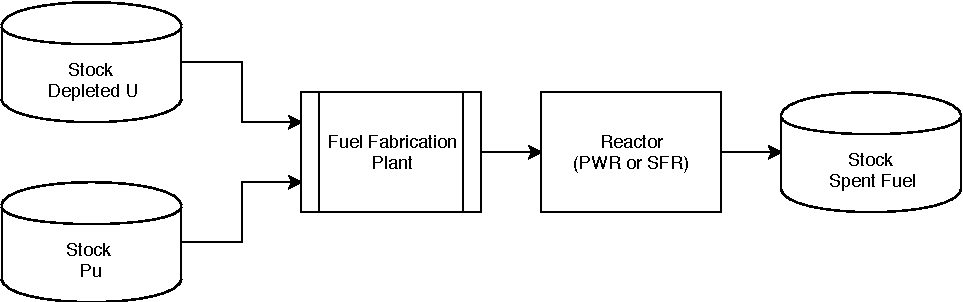
\includegraphics[width = 0.99\textwidth]{FIG/FuelCycleDiagram.pdf}
        \caption{Representation of the simulated fuel cycle facilities.}
        \label{fig:FuelCycle}
    \end{center}
\end{figure}

The time frame of the simulation corresponds to the reactor cycle. From the relation between the fuel cycle time $\Delta t$, the reactor thermal power $P_{th}$, the heavy nuclide mass $M$ and the reactor burn-up $BU$, we have : 

\begin{equation}
    \Delta t = \frac{BU \; M}{P_{th}}
\end{equation}

At t = 0, the fabrication plant builds the fresh fuel according to reactor requirements. To avoid plutonium isotopes decay, the fabrication time is zero and the reactor is thus loaded instantaneously. A complete fuel cycle is run and the spent fuel is sent to stock when the required BU is reached.

In the framework of this exercise, the plutonium vector has to be ranged in order to be representative 

Pas la pour étudier des scénarios très contraint et donc très tuné... Pour un scénario très contraint, FF is clearly enough. Pas la peine de passer du temps pour développer un FLM

Scenario exploratoire donc plein de possibilité
Candu avec Pu9 pur
PWR mono et multi mox
SFR symbiotic 
Temps de refroidissement variable et decay du Pu241

Donc super large!


The plutonium vectors that could be tested in the framework of this exercise have to be "realistic". We propose the following table with minimum and maximum isotopic fraction and total fraction in the fuel. 

Isotope Min. Fraction (wgt. %)  Max. Fraction (wgt. %)
Pu/HM @ T0 (PWR)    5   10
Pu/HM @ T0 (SFR)    13  22
Pu-238/TRU  0   10
Pu-239/TRU  25  90
Pu-240/TRU  10  40
Pu-241/TRU  0   25
Pu-242/TRU  0   30
Am-241/TRU  0   10

Each user can use a different plutonium vector as long as it is included inside this range


% -----------------------------------------------------------------------------------------
\subsection{Methodology}

In order to investigate the influence of fuel fabrication models on fuel cycle
simulations, the following experiment have been designed. Following the FIT
project spirit, no code to code comparison will be done. For each simulator used
to solve this problem, fuel models will be compared within the same simulator,
allowing to evaluate difference between two almost identical simulation: same
simulator, reactor description, depletion algorithm, \ldots the only difference
being the fuel fabrication model used.

The experiment consists in running a small fuel cycle, composed by a infinite
plutonium source, a fuel fabrication and a reactor, for multiple plutonium
isotopic compositions (about 1000). Each plutonium isotopic will be run twice,
one using a fuel fabrication model using a fixed fraction, always the same
defined in the experiment specification, and a second one using an advanced fuel
loading model (based on plutonium equivalent theory\ref{} or pre-trained neural
networks).

The different plutonium composition are sampled uniformly on a predefined
user-space (that may vary depending of the simulator used). Moreover, even if
it is understood that an largely under/over-estimated plutonium content in the
MOX fuel, may compromise the reactor well operation, it is assumed in the
following that all fuel loading models used (fixed fraction or more complex fuel
loaded models), will produced proper MOX fuels.

In order to measure the influence of the used of fixed fraction versus a fuel
loading models on the global amount of plutonium in the simulation, the location
of the plutonium and the speed of variation of the plutonium inventory, three
estimators have been defined.

\subsection{Estimators}
\subsubsection{Estimator 1}
The first estimator aims to the difference on the plutonium enrichment in the MOX
fuel between the \gls{FLM} and \gls{FF} which directly impacts the amount of
plutonium present in the back-end part of the fuel cycle. The estimator 1 has
been defined as:
\begin{equation}
    \delta{\lambda}(i) =
        \frac{\left(\lambda_{\mathrm{Pu}}^{BOC}(i)\right)_{FML}
              - \left(\lambda_{\mathrm{Pu}}^{BOC}(i)\right)_{FF}}
              {\left(\lambda_{\mathrm{Pu}}^{BOC}(i)\right)_{FF}},
\end{equation}

where $\lambda_i$ represents the fraction of plutonium at \gls{BOC} or at
\gls{EOC} for the plutonium composition $i$ for the \gls{FLM} or the \gls{FF}.

\subsubsection{Estimator 2}
The second estimator aims to relative speed of plutonium amount evolution in the
reactor between the \gls{FLM} and the \gls{FF}. The estimator 2 is defined as:
\begin{equation}
    \delta{\frac{\Delta M}{M}}(i) =
        \frac{\left(\frac{\Delta M}{M}(i)\right)_{FML}
              - \left(\frac{\Delta M}{M}(i)\right)_{FF}}
             {\left(\frac{\Delta M}{M}(i)\right)_{FF}},
\end{equation}
where $\frac{\Delta M}{M}_{i}$ is defined as:
\begin{equation}
    \frac{\Delta M}{M}(i) = \frac{M_{Pu}^{BOC}(i) -
    M_{Pu}^{EOC}(i)}{M_{Pu}^{BOC}(i)}
\end{equation}


\subsubsection{Estimator 3}


\begin{equation}
    \delta{\frac{\Delta M}{T}}(i) =
        \frac{\left(\frac{\Delta M}{T}(i)\right)_{FML}
              - \left(\frac{\Delta M}{T}(i)\right)_{FF}}
             {\left(\frac{\Delta M}{T}(i)\right)_{FF}},
\end{equation}
where $\frac{\Delta M}{T}_{i}$ is defined as:
\begin{equation}
    \frac{\Delta M}{T}(i) = \frac{M_{Pu}^{BOC}(i) -
    M_{Pu}^{EOC}(i)}{T}
\end{equation}

% -----------------------------------------------------------------------------------------
\subsection{Output observables}



% coucou

\section{Results}
 
\subsection{Pressurized Water Reactor}

\subsubsection{Output analyses}
Figure~(\ref{fig:PWR_MOX_FLM_Pu.pdf}) presents the plutonium fraction at BOC predicted by each FLM and the plutonium fraction at EOC deduced by each software. As all FLM are different, the BOC plutonium fractions differ from a software from another. The wider prediction is given by the CLASS code that predicts plutonium fraction from 4\% until more that 15\%. This range is a direct consequence of the plutonium sampling used for this work. 15\% is clearly unrealistic but some of the plutonium isotopic composition sampled are not eather by containing a low amount of fissile. That'is why the FLMs may reach such high values.   

\begin{figure}[h]
	\begin{center}
		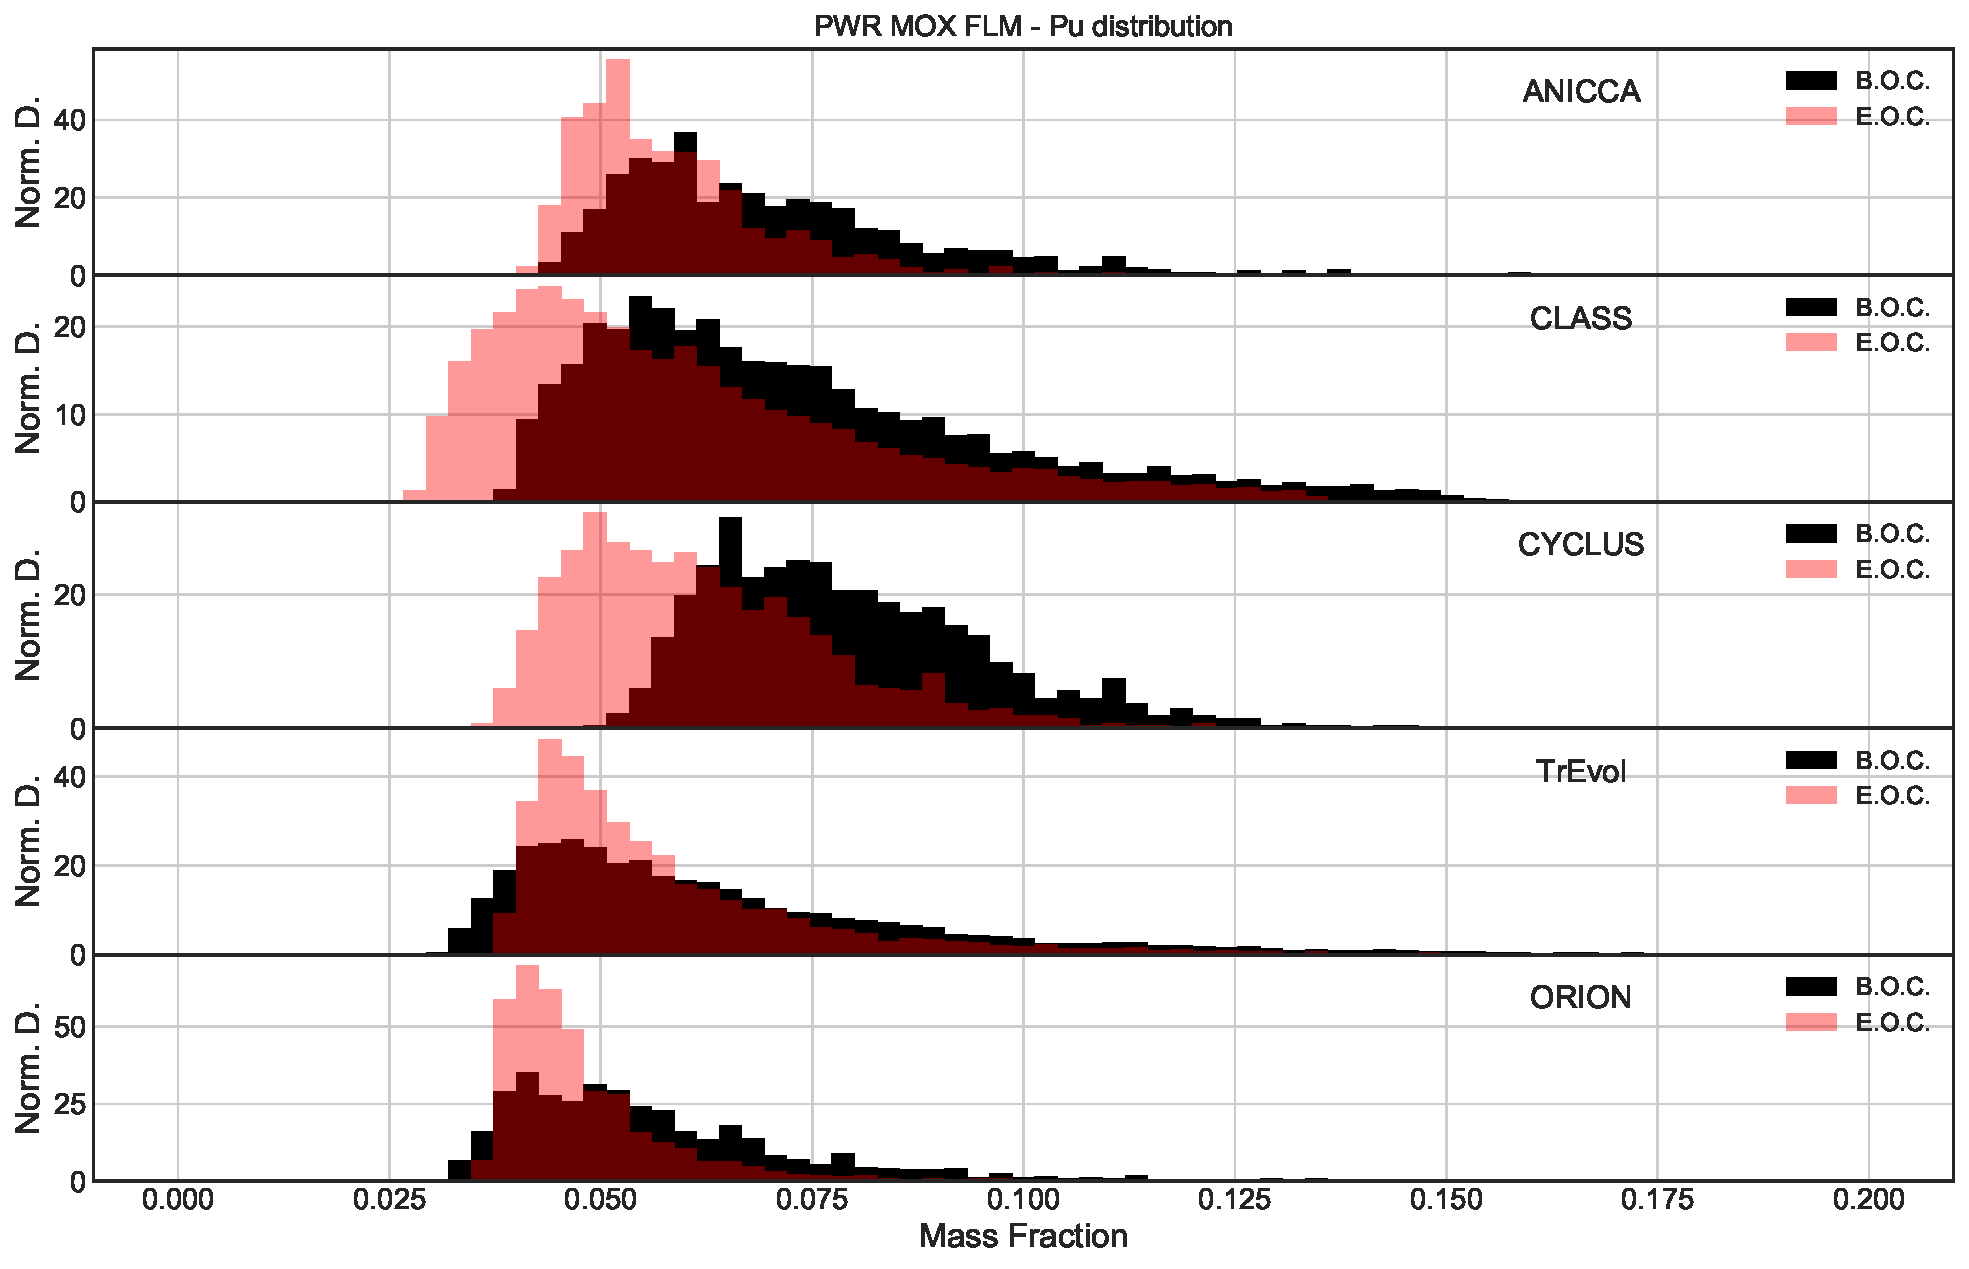
\includegraphics[width = 0.8\textwidth]{../../Feature_1/RAW_DATA/FIG/PWR_MOX_FLM_Pu.pdf}
		\caption{Code outputs for PWR scenario's calculations}
		\label{fig:PWR_MOX_FLM_Pu.pdf}
	\end{center}
\end{figure}

The EOC plutonium fraction is clearly shiffted to the lower values, proving that plutonium is consumed during irradiation like it should be in PWRs.   

\subsubsection{Estimator's calculation}

Figure~(\ref{fig:Est1_PWR}), figure~(\ref{fig:Est2_PWR}) and figure~(\ref{fig:Est3_PWR}) presents the calculation results for PWR of the different estimators defined in the previous section. Estimator 1 aims to quantify biais introduced by the use of a FF model on the plutonium enrichment for fresh MOX fuel. It measures the amount of plutonium taken from UOX spent fuel for MOX fuel fabrication. As it can be seen, 

\begin{figure}[h]
	\begin{center}
		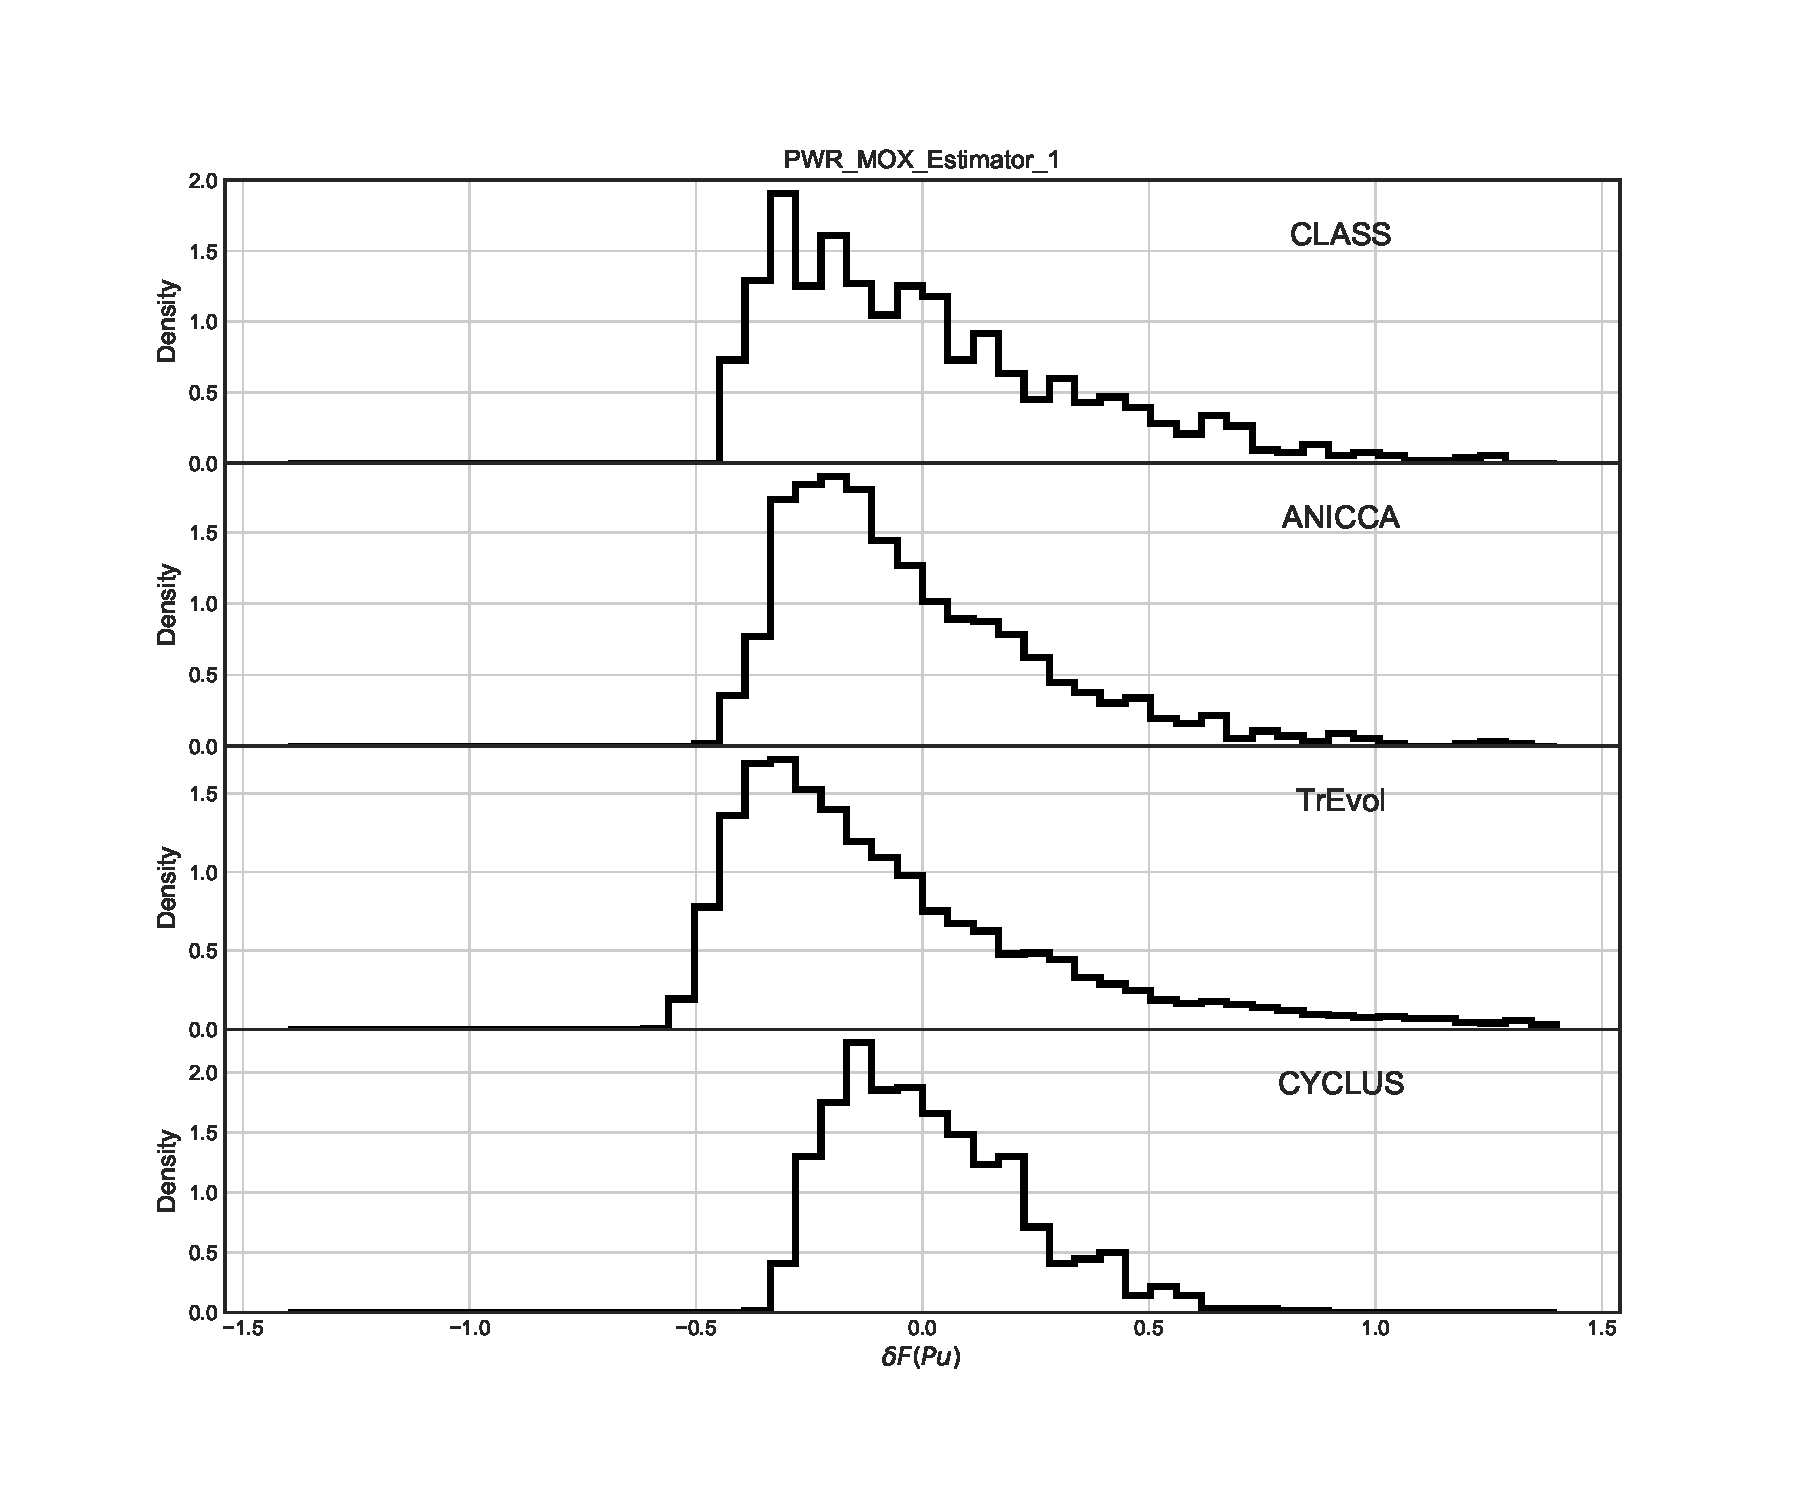
\includegraphics[width = 0.8\textwidth]{../../Feature_1/RAW_DATA/FIG/PWR_MOX_Estimator_1.pdf}
		\caption{Estimator 1 for PWR calculated with ANICCA, CLASS, CYCLUS and TrEVOL}
		\label{fig:Est1_PWR}
	\end{center}
\end{figure}


\begin{figure}[h]
	\begin{center}
		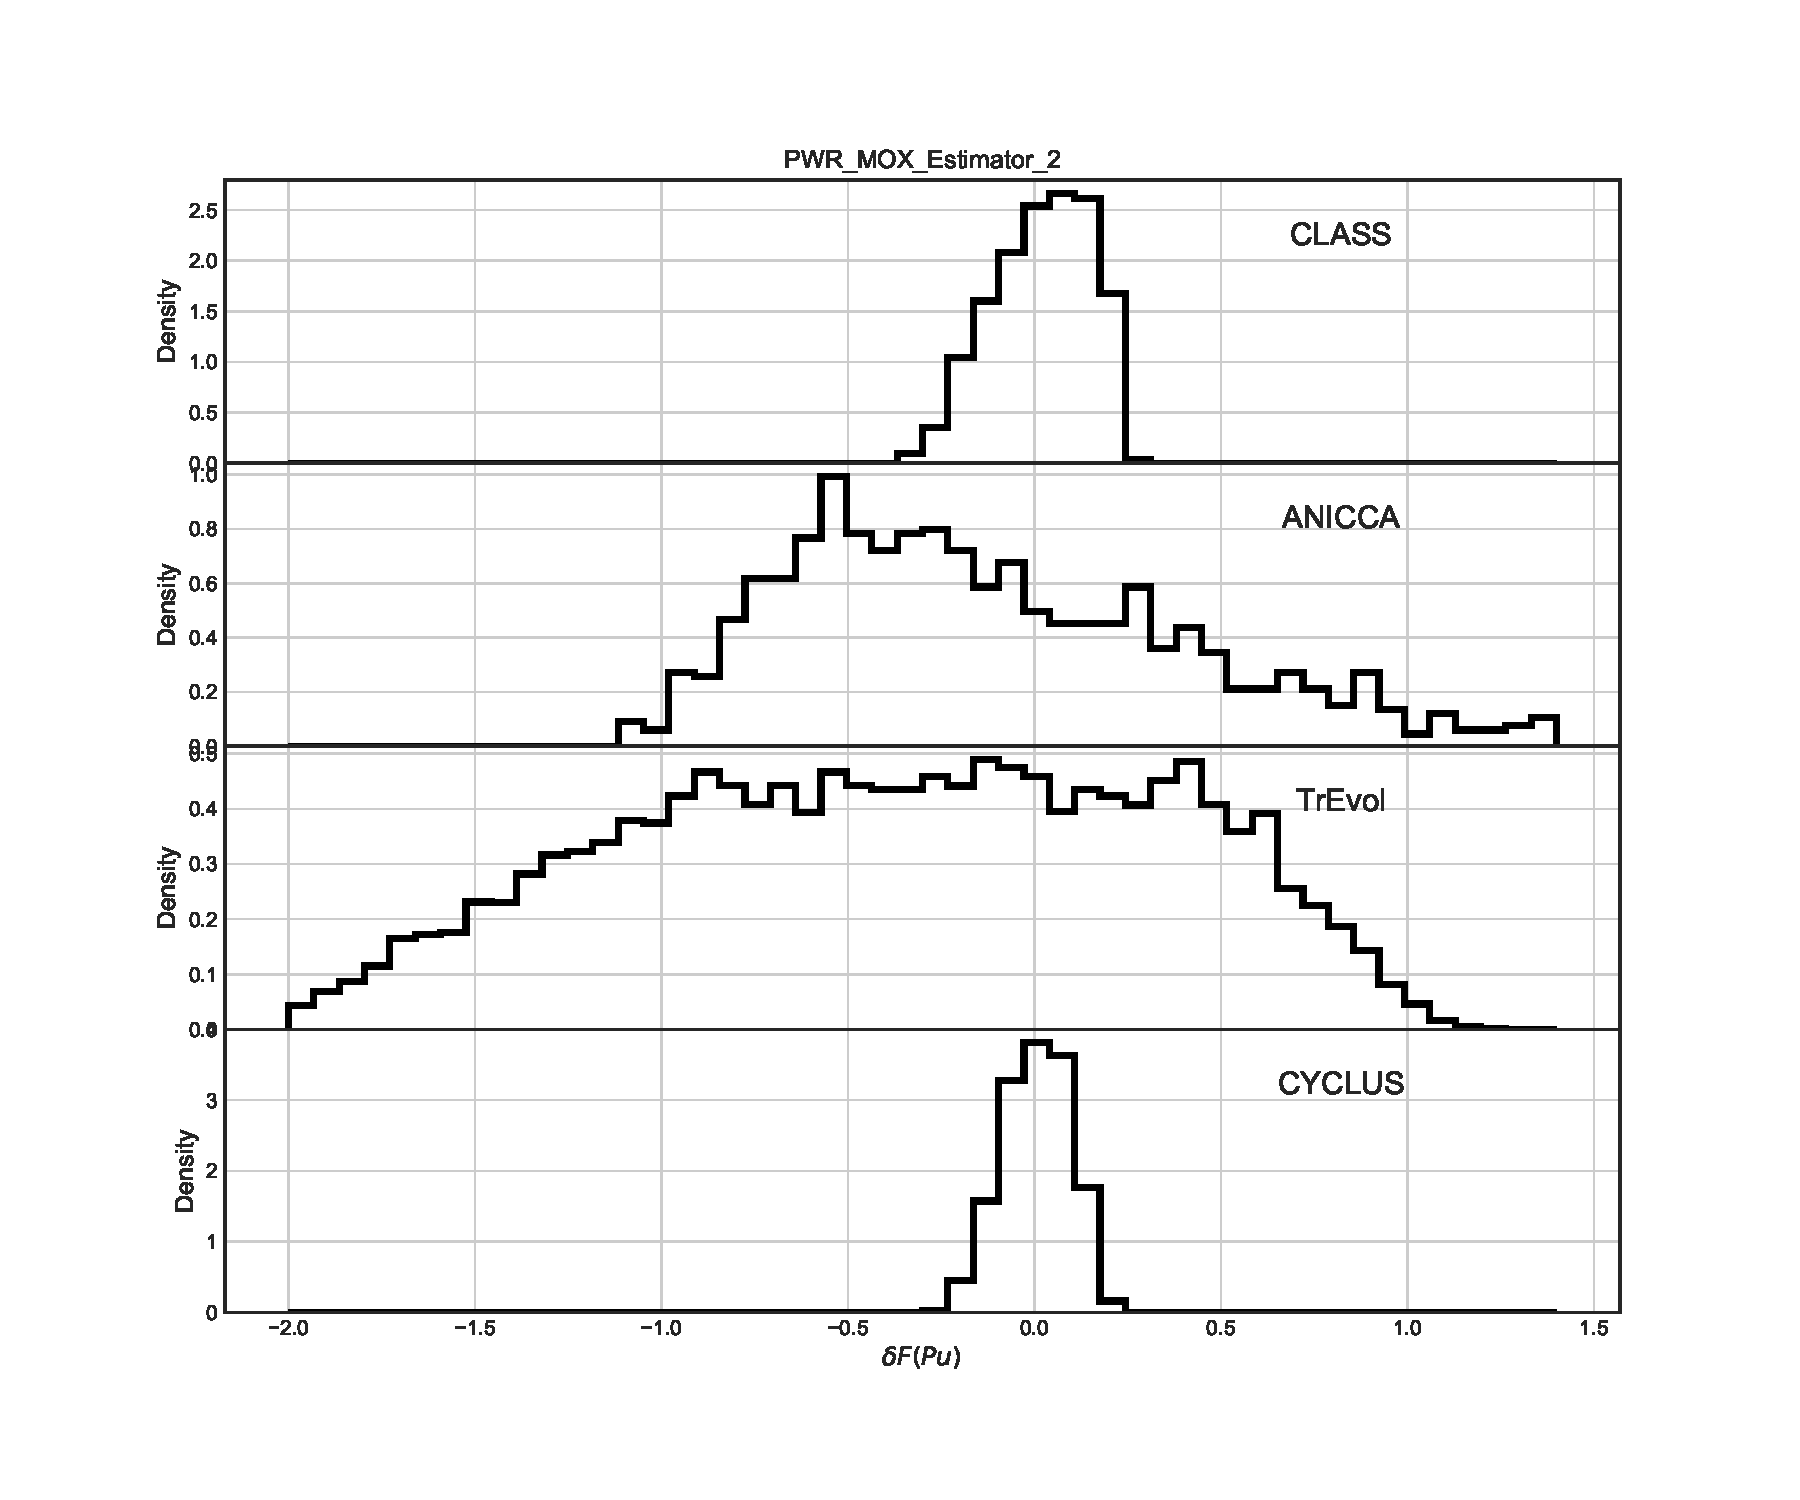
\includegraphics[width = 0.8\textwidth]{../../Feature_1/RAW_DATA/FIG/PWR_MOX_Estimator_2.pdf}
		\caption{Estimator 2 for PWR calculated with CLASS, CYCLUS and TrEVOL}
		\label{fig:Est2_PWR}
	\end{center}
\end{figure}

\begin{figure}[h]
	\begin{center}
		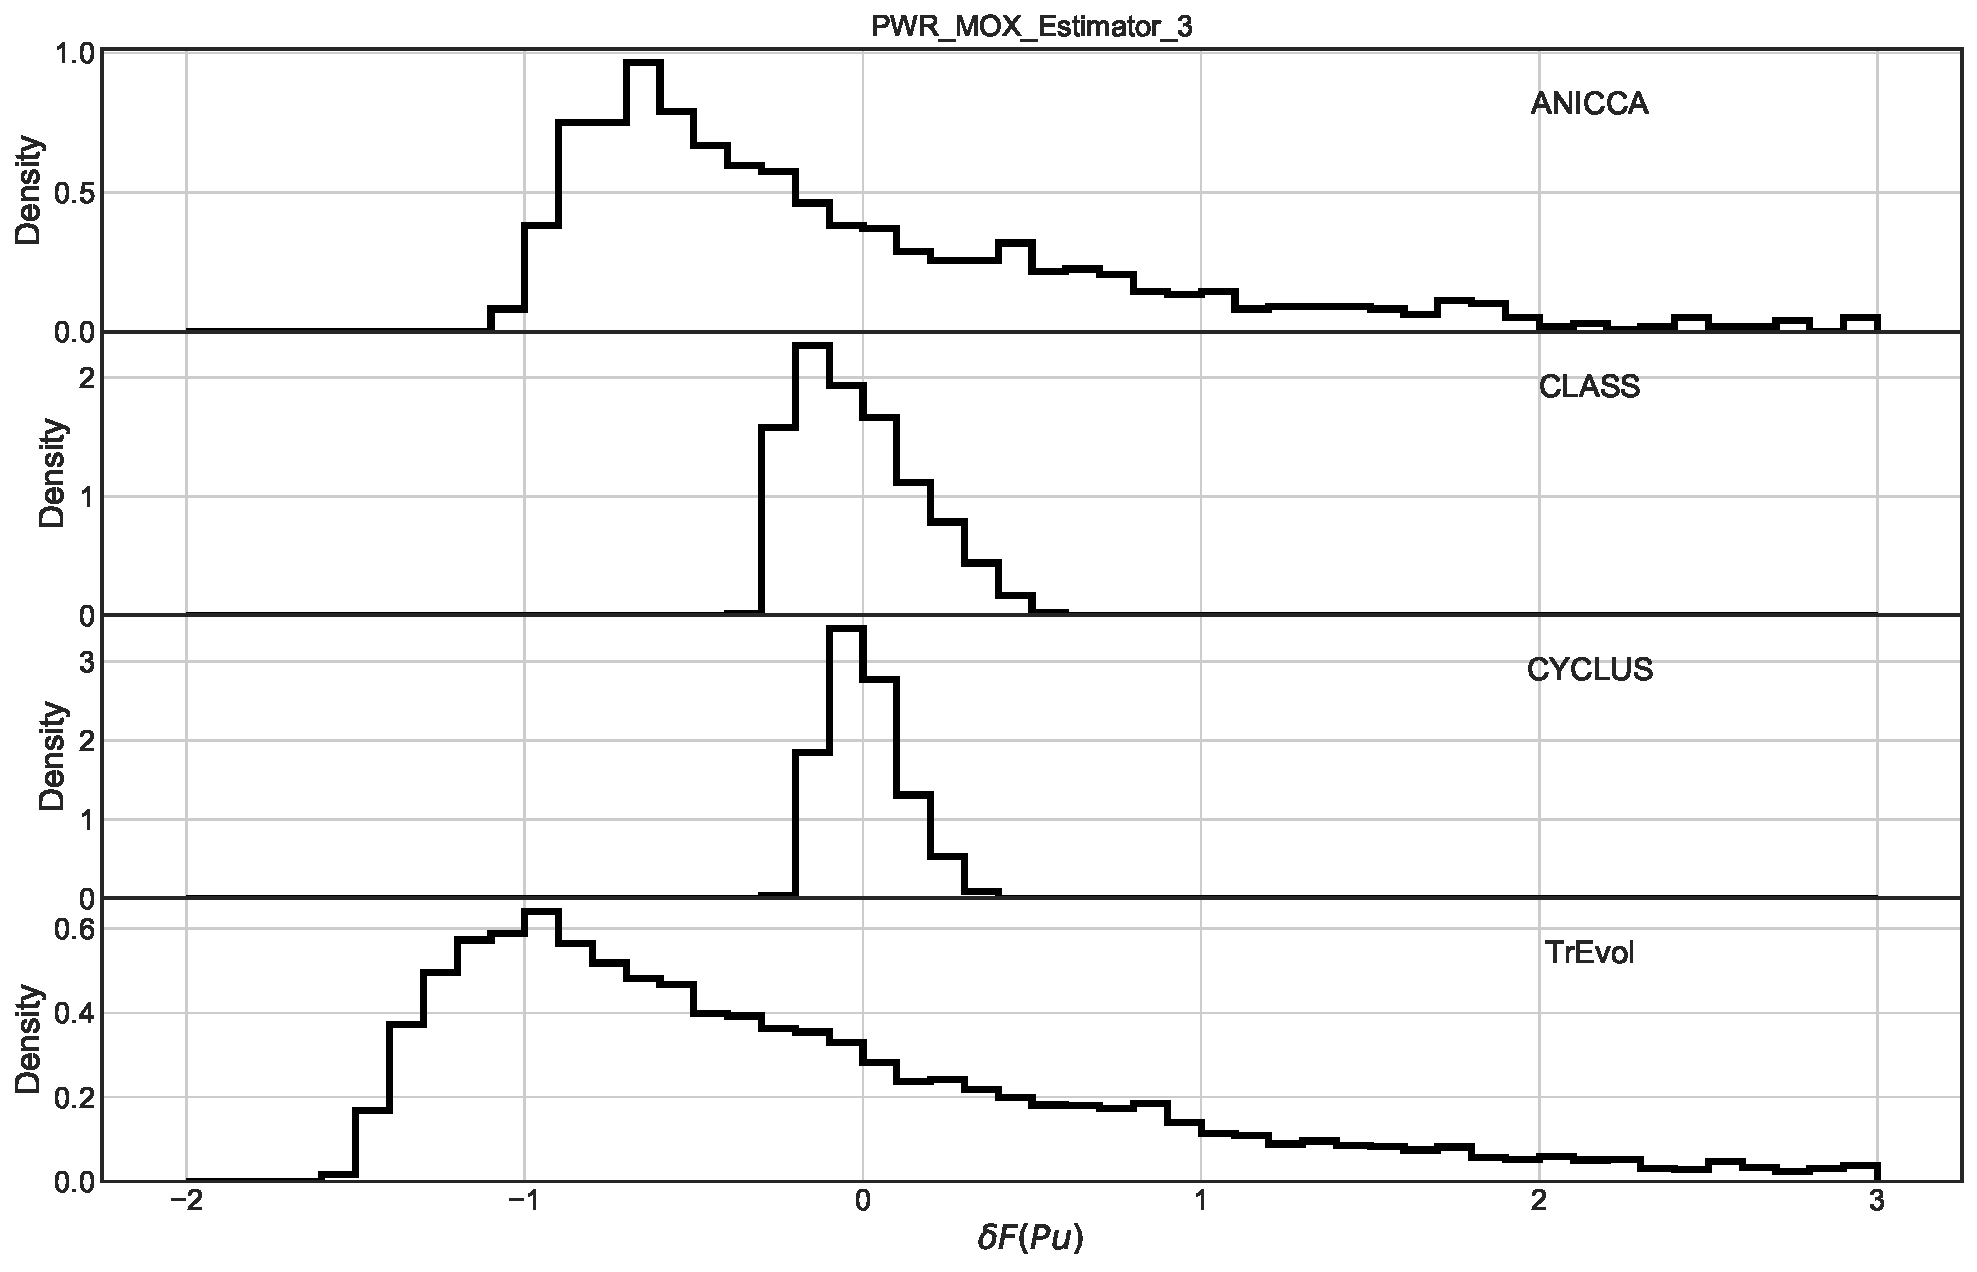
\includegraphics[width = 0.8\textwidth]{../../Feature_1/RAW_DATA/FIG/PWR_MOX_Estimator_3.pdf}
		\caption{Estimator 3 for PWR calculated with CLASS, CYCLUS and TrEVOL}
		\label{fig:Est3_PWR}
	\end{center}
\end{figure}

\subsection{Fast Sodium cooled Reactor}

Figure~(\ref{fig:Est1_SFR}) represents the estimator 1 calculated for Sodium Cooled Fast Reactors calculated with JOSETTE, TrEVOL and CLASS. Like for PWR, it shows the relative difference of plutonium enrichment with the use of a FLM in regards to a FF. Standard deviations of the difference distribution is given in table~(\ref[table:Est1Dev_SFR]) for the different codes. 
All codes are in agreement even if CLASS slightly underestimate the FF impact on the plutonium needed for a SFR. The typical biais produced by the use of a FF is smaller than 25\% and is much lower than for PWR.  

\begin{figure}[h]
	\begin{center}
		\includegraphics[width = 0.8\textwidth]{}
		\caption{Estimator 1 for SFR calculated with JOSETTE, TrEVOL, and CLASS}
		\label{fig:Est1_SFR}
	\end{center}
\end{figure}

\begin{table}[h]
	\begin{center}
		\begin{tabular}{|c||c||c|}
			\hline 
				JOSETTE & TrEVOL & CLASS
			\hline
				XX & YY & ZZ 
		\end{tabular}
	\end{center}
	\label{table:Est1Dev_SFR}
\end{table}

\begin{figure}[h]
	\begin{center}
		\includegraphics[width = 0.8\textwidth]{}
		\caption{Estimator 2.b for SFR calculated with JOSETTE, TrEVOL, and CLASS}
		\label{fig:Est2_SFR}
	\end{center}
\end{figure}


% #########################################################################################
% #########################################################################################
% #########################################################################################
\section*{References}

\bibliography{mybibfile}

\end{document}
